\documentclass[letterpaper]{article}

\usepackage[cm,plain]{fullpage}

\usepackage{algorithm}
\usepackage{algorithmic}
\usepackage{amsmath}
\usepackage{amssymb}
\usepackage{graphicx}

\usepackage{subfigure}

\usepackage{color}
\usepackage{hyperref}
\usepackage{url}

\definecolor{col}{rgb}{1.0,0.27,0.0}

\linespread{1.3}

\let\oldthebibliography=\thebibliography
\let\endoldthebibliography=\endthebibliography
\renewenvironment{thebibliography}[1]{%
  \begin{oldthebibliography}{#1}%
    \setlength{\parskip}{0ex}%
    \setlength{\itemsep}{0ex}%
}%
{%
  \end{oldthebibliography}%
}

\begin{document}

\title{\vspace{-120pt}}

%\author{}
%\date{}

%\maketitle

\begin{figure}[h]
\begin{center}
\subfigure[\label{fig:car-tube1}]{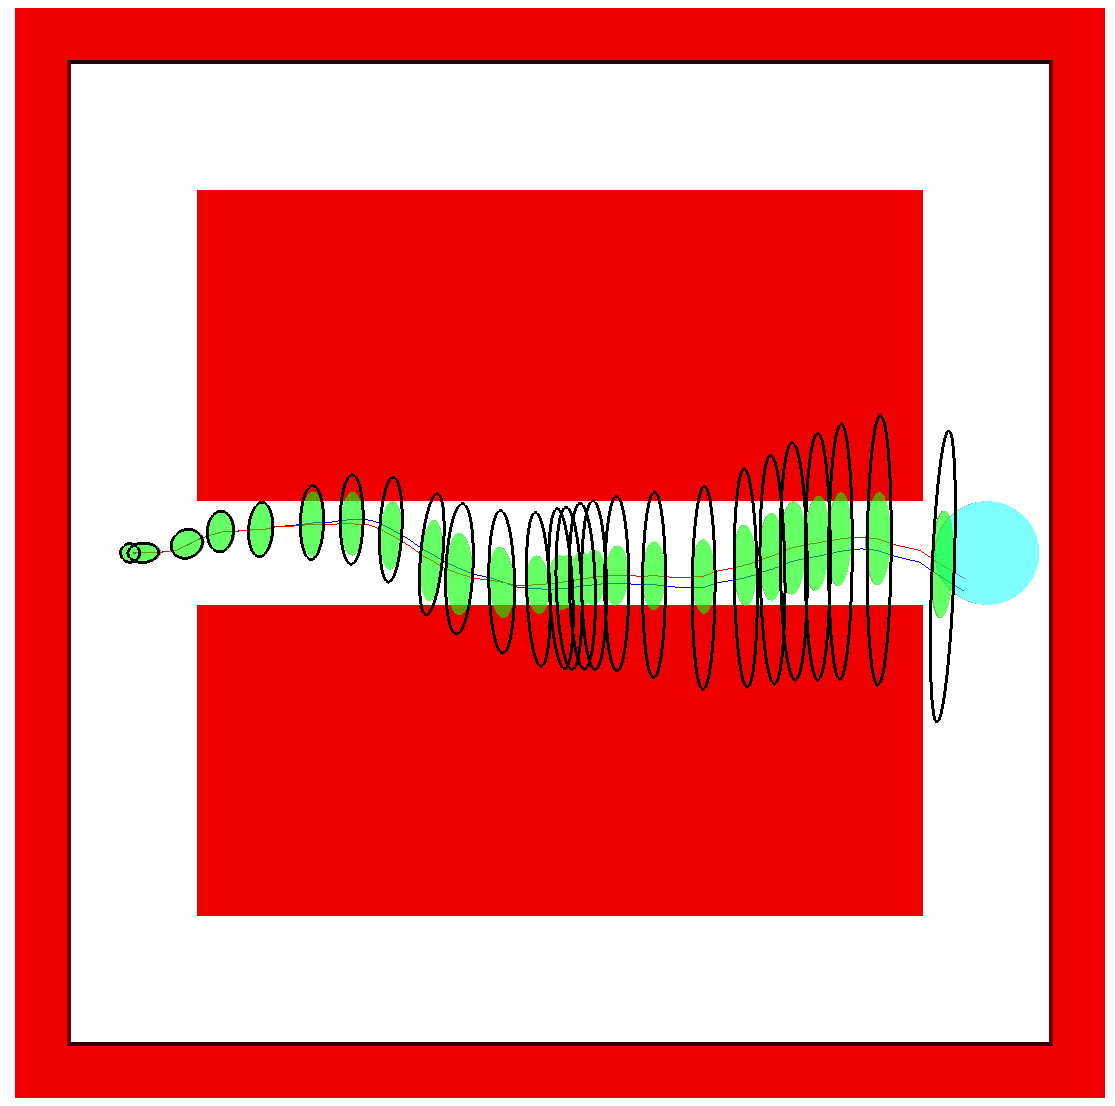
\includegraphics[width=0.49\linewidth]{figures/working/car-tube1.png}}
\subfigure[\label{fig:car-tube1-trunc}]{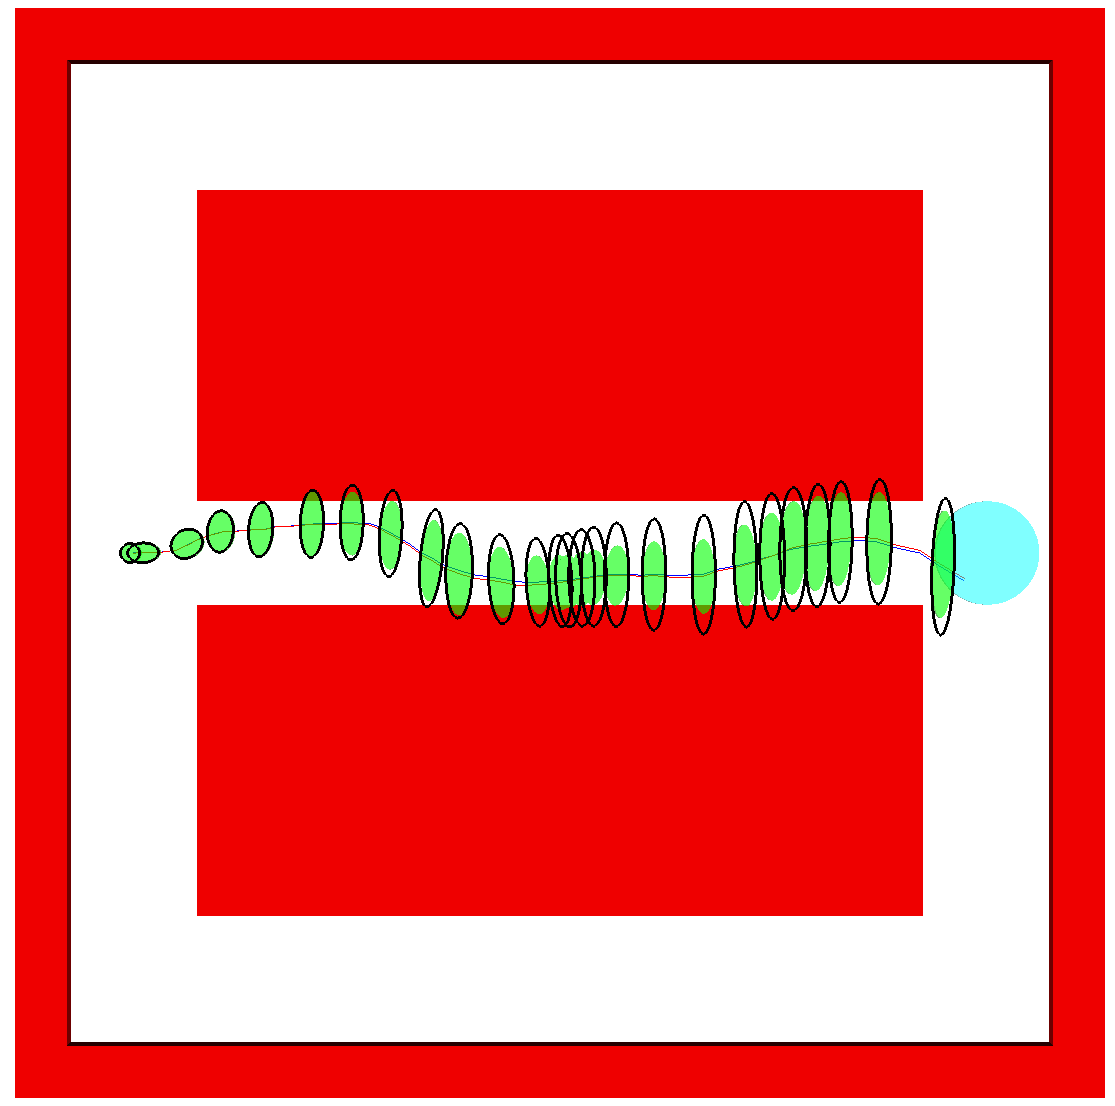
\includegraphics[width=0.49\linewidth]{figures/working/car-tube1-trunc.png}}\\
\subfigure[\label{fig:car-tube2}]{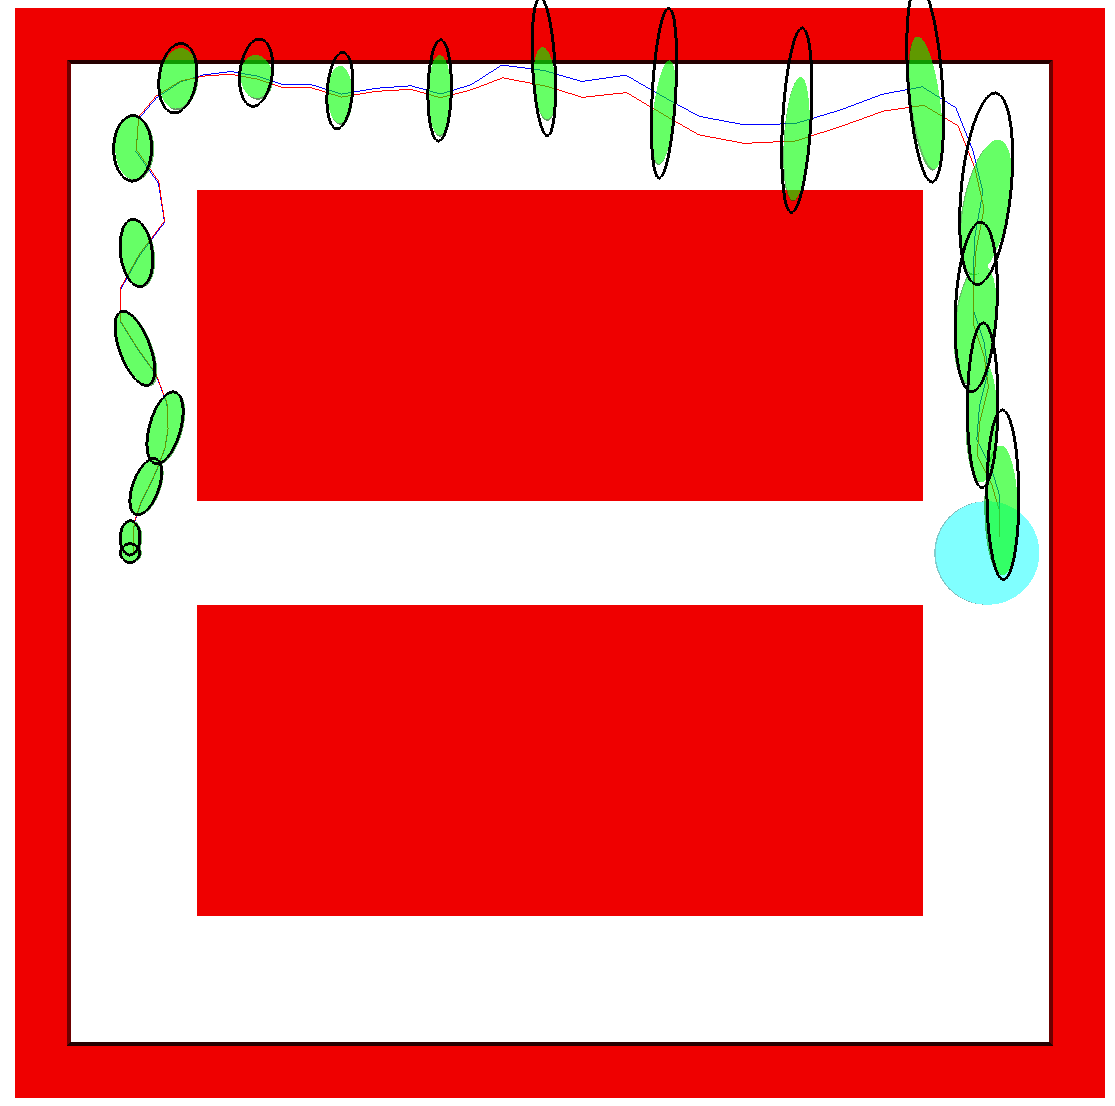
\includegraphics[width=0.49\linewidth]{figures/working/car-tube2.png}}
\subfigure[\label{fig:car-tube2-trunc}]{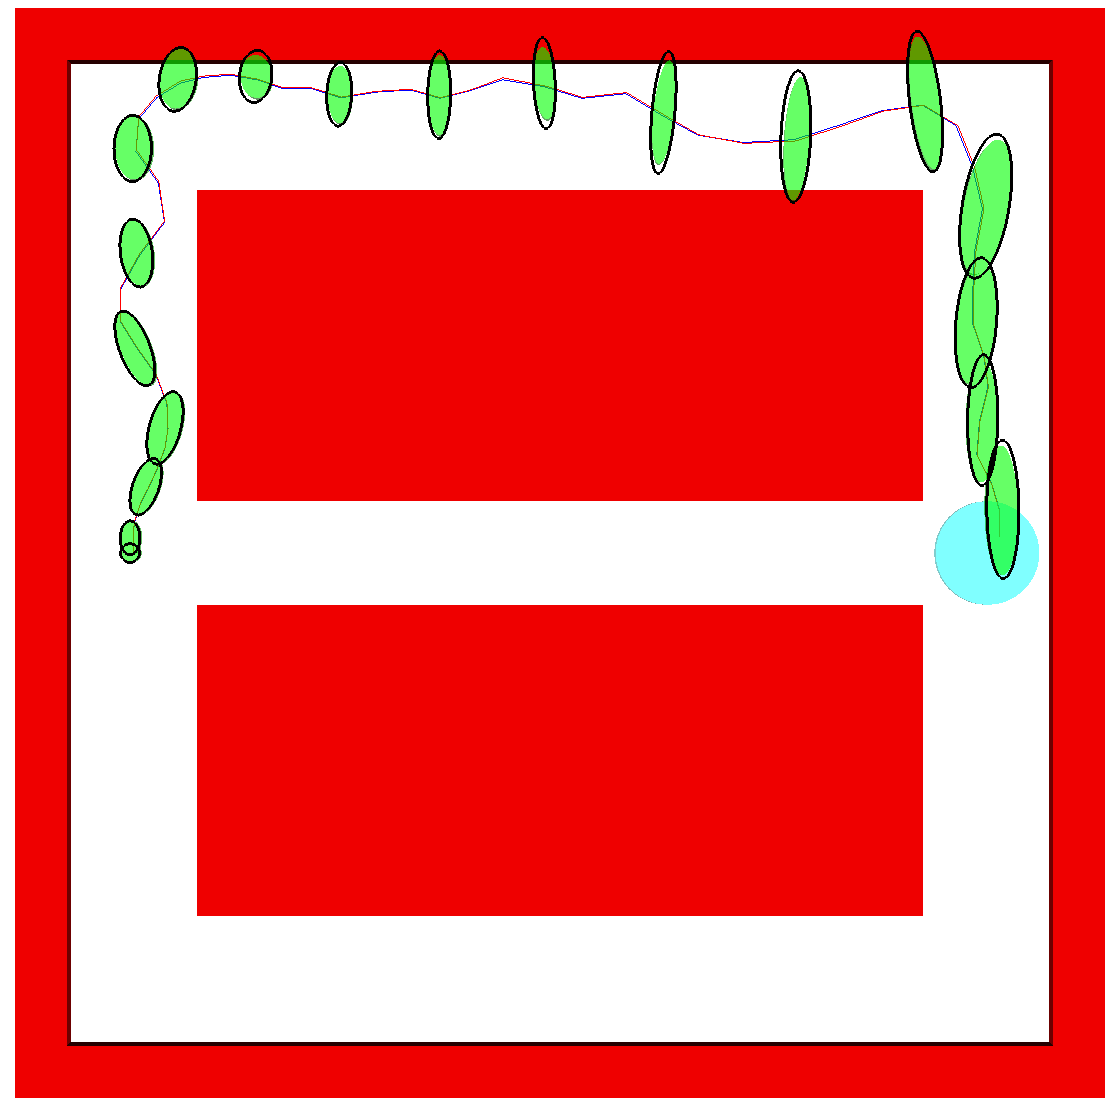
\includegraphics[width=0.49\linewidth]{figures/working/car-tube2-trunc.png}}\\
\vspace{-20pt}
\end{center}
\caption{ Full 4D nonlinear car dynamics model (from LQG-MP paper). The a priori distributions computed by truncating and propagating LQG-MP covariances (green) and Gaussian distribution of $100000$ samples (black) at each time-step. The red poly-line is the mean path of the truncation method and the blue poly-line is the mean path computed by sampling. [a,b] Truncating and propagating LQG-MP covariances underestimates the maximum likelihood distribution (black) for this particular case (Why?). [c,d] Almost identical.}
\label{fig:panel1}
\end{figure}

\begin{figure}[h]
\begin{center}
\subfigure[\label{fig:car-path1}]{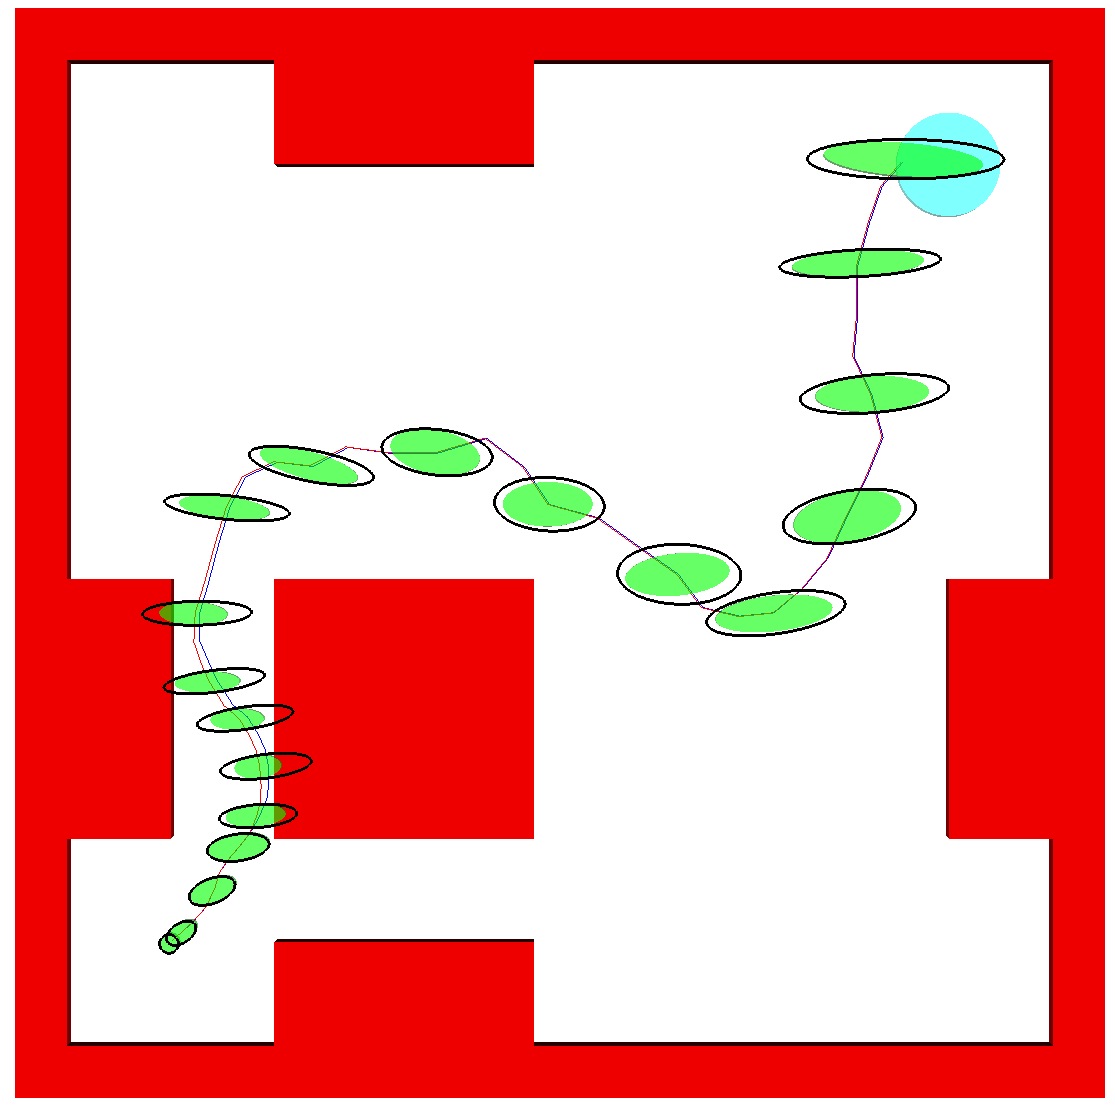
\includegraphics[width=0.49\linewidth]{figures/working/car-path1.png}}
\subfigure[\label{fig:car-path1-trunc}]{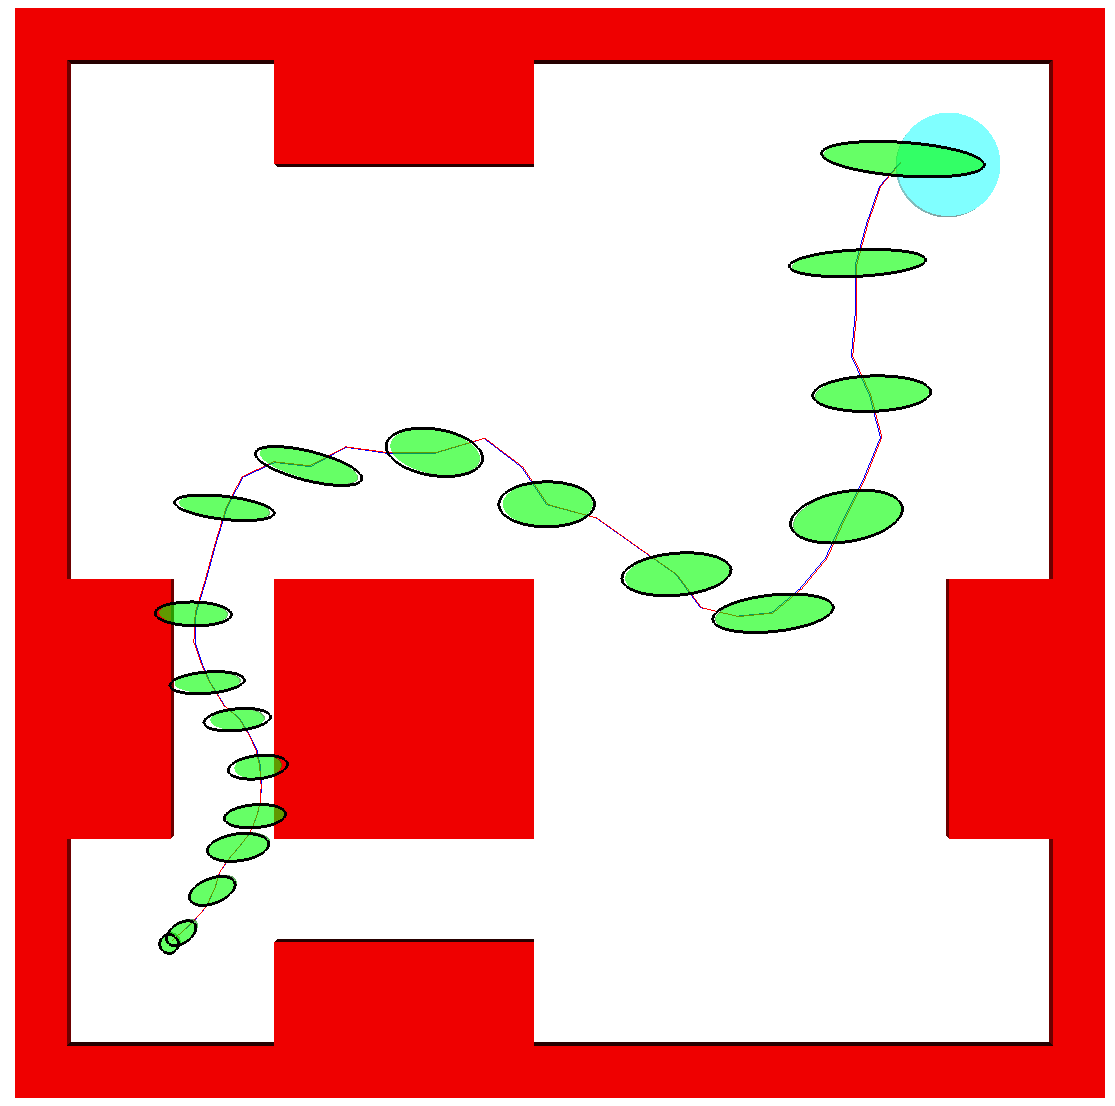
\includegraphics[width=0.49\linewidth]{figures/working/car-path1-trunc.png}}\\
\subfigure[\label{fig:car-path2}]{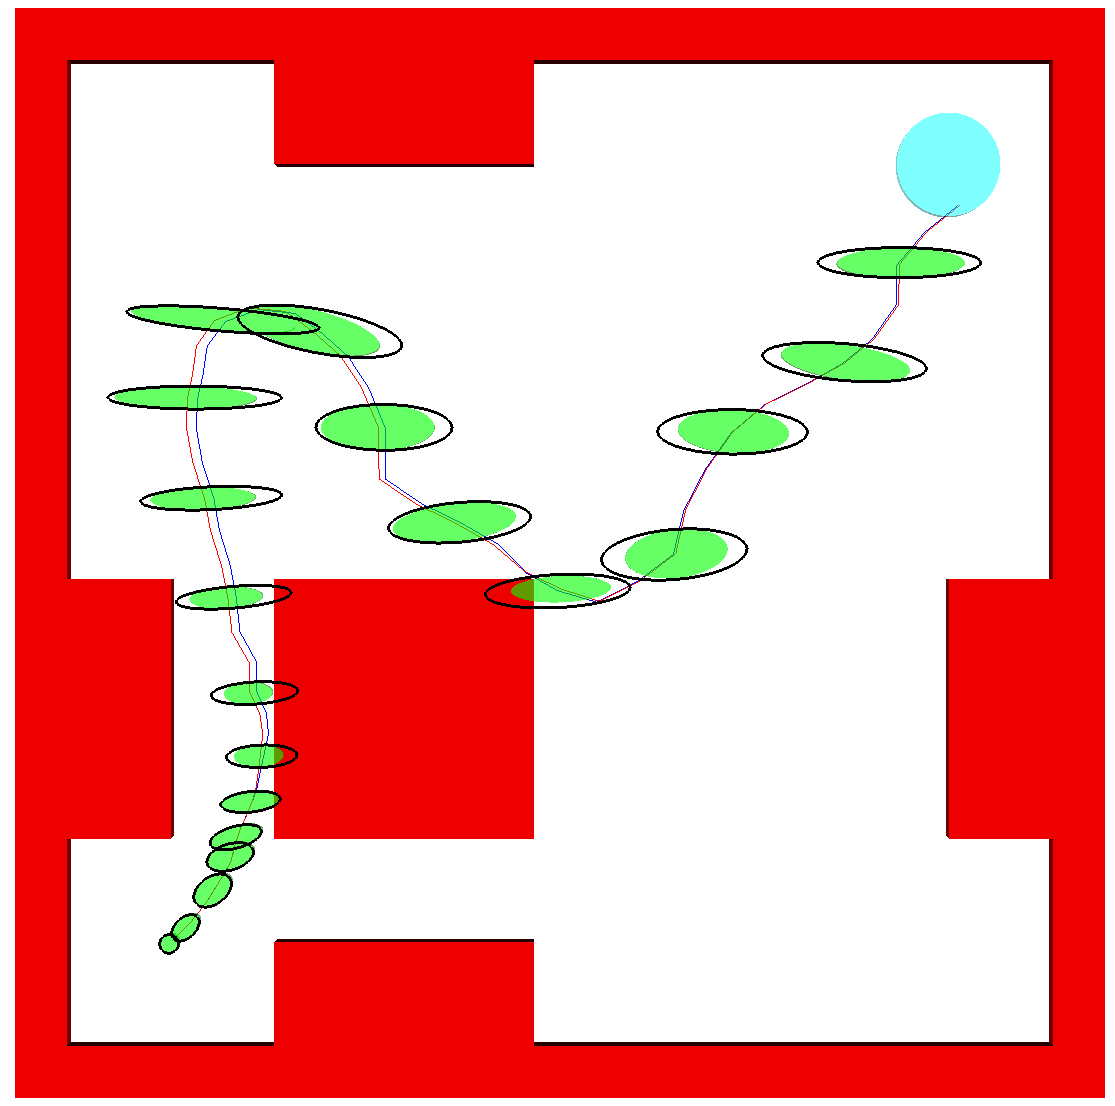
\includegraphics[width=0.49\linewidth]{figures/working/car-path2.png}}
\subfigure[\label{fig:car-path2-trunc}]{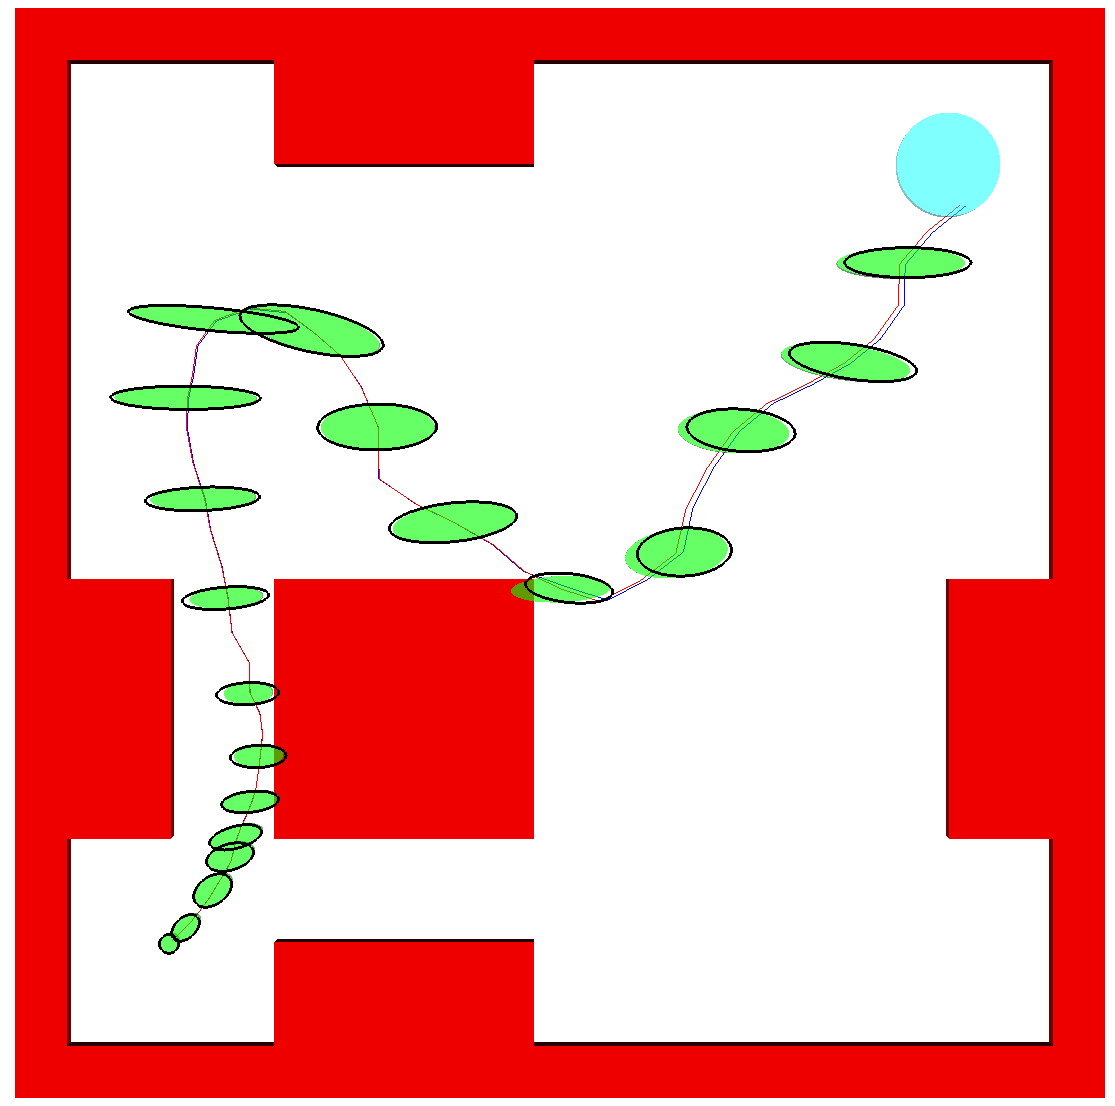
\includegraphics[width=0.49\linewidth]{figures/working/car-path2-trunc.png}}\\
\vspace{-20pt}
\end{center}
\caption{ [a,b] Almost identical. [c,d] Notice how the distribution towards the corner of the obstacle in the middle is computed incorrectly, causing discrepancies further down the path. This is most likely an artifact of the convex decomposition.}
\label{fig:panel1}
\end{figure}

\begin{figure}[t]
\begin{center}
\subfigure[\label{fig:point2d}]{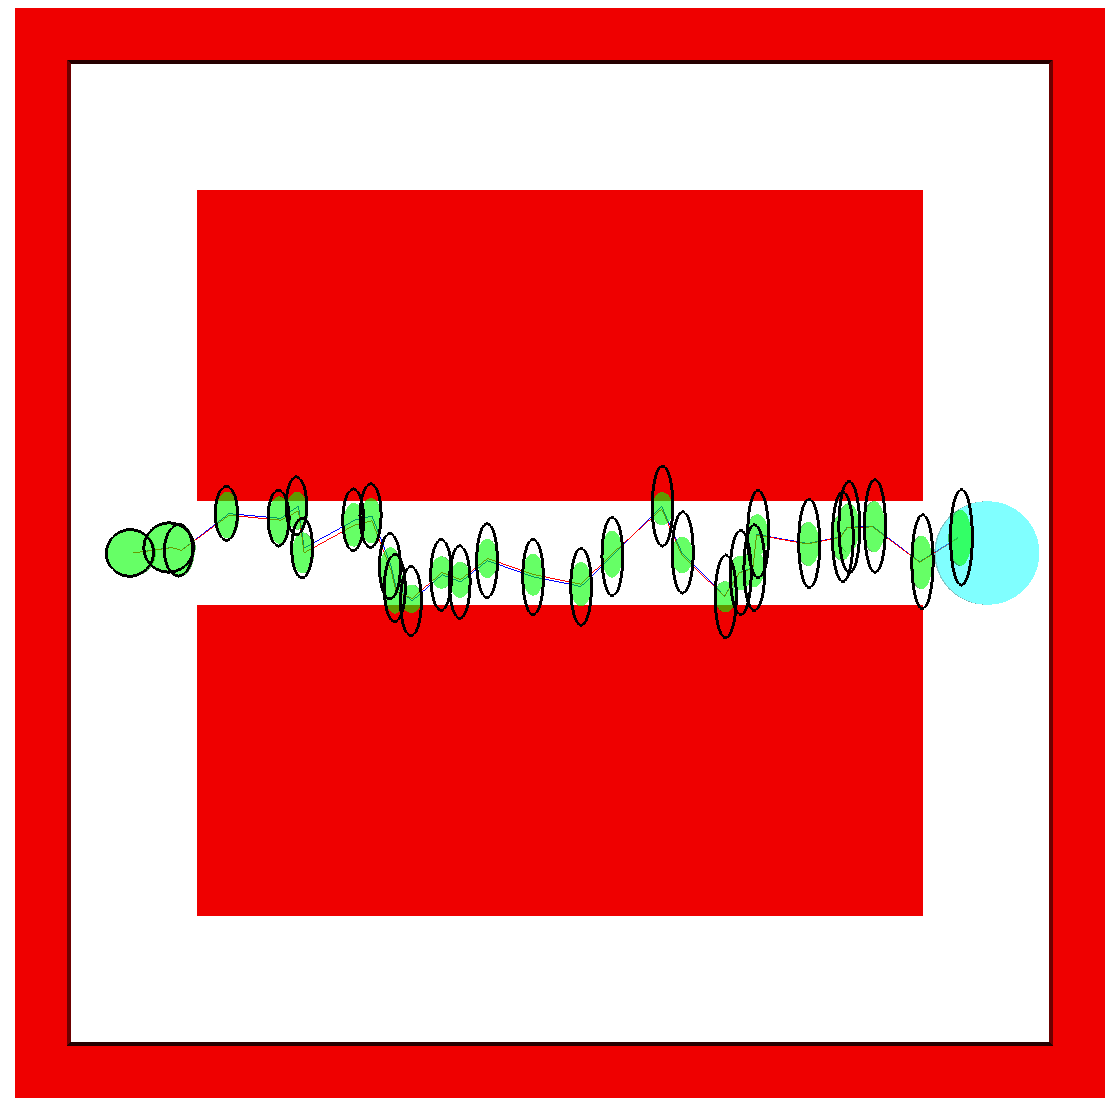
\includegraphics[width=0.49\linewidth]{figures/working/point2d.png}}
\subfigure[\label{fig:point2d-trunc}]{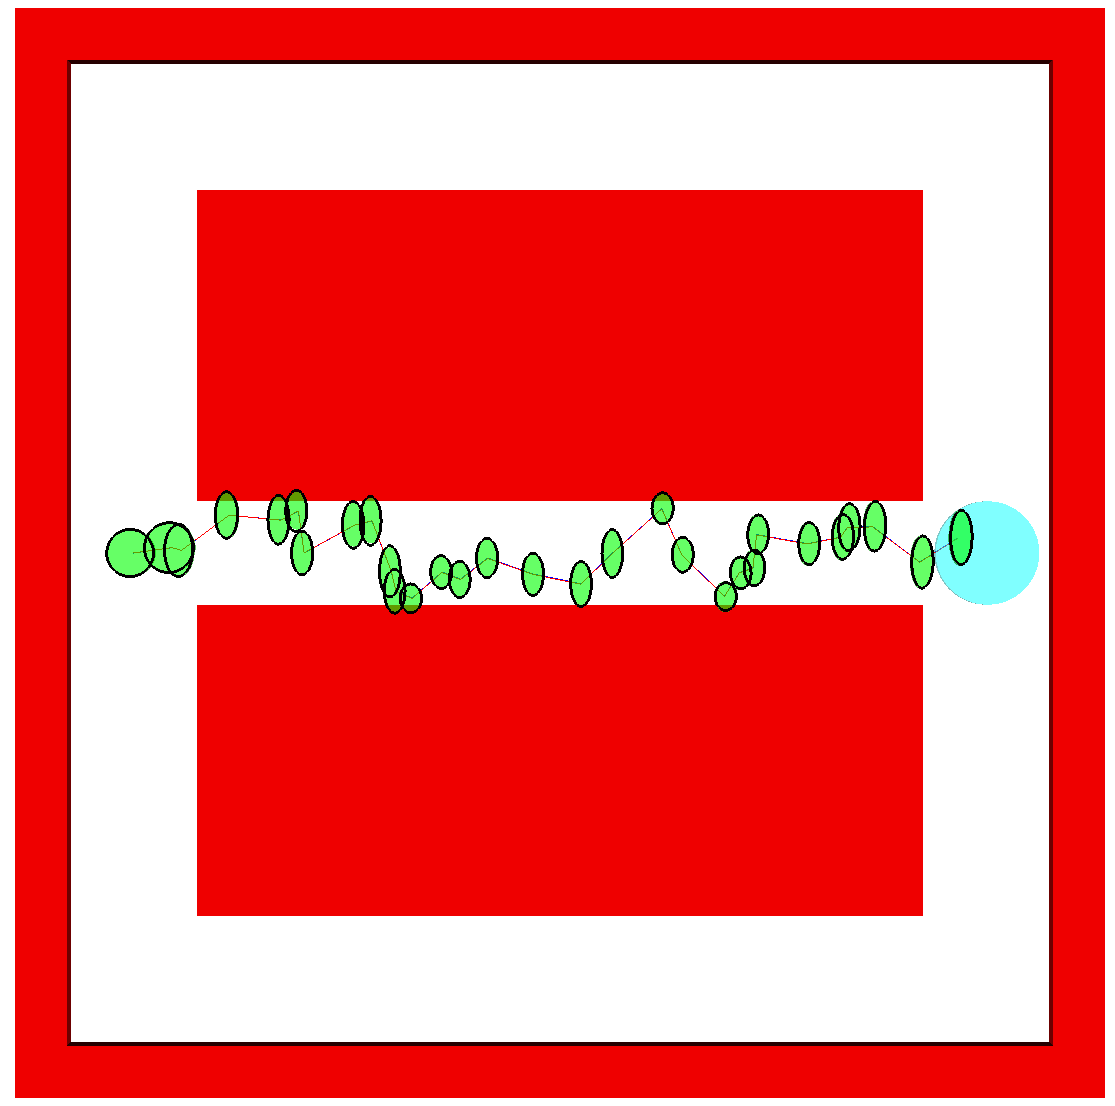
\includegraphics[width=0.49\linewidth]{figures/working/point2d-trunc.png}}
\vspace{-20pt}
\end{center}
\caption{ Simple 2D holonomic robot: [a,b] Identical.}
\label{fig:panel4}
\end{figure}

\end{document} 